\paragraph{}
Um den Nutzern eine ansprechende Benutzeroberfläche zu bieten, durch die der Klient über eine Schnittstelle mit dem Server kommunizieren und schlussendlich unsere Webseite bedienen kann, ist eine Mehrzahl an ineinandergreifenden Technologien (eng.: Techstack) notwendig.

\paragraph{}
Es wurde sich für MERN entschieden, einem ausgereiften Techstack bestehend aus MongoDB als Datenbank, NodeJS und Express im Backend und React im Frontend.
Diese Technologien eignen sich für die Entwicklung von Webapplikationen mit hoher Qualität und erlaubt eine schnelle Entwicklung \cite{ti:mernStackAdvantages}.
Alle genannten Technologien verwenden die Programmiersprache JavaScript.
Dies erleichtert das Programmieren, da nicht zwischen den Syntaxen verschiedener Sprachen gewechselt werden muss.
Auch kann der gleiche Programmiercode an verschiedenen Stellen des Projektes wiederverwendet werden, was Zeit und Kosten spart.
Die Technologien sind ausgereift und werden vielfach aktiv von führenden Technologiegiganten verwendet \cite{ti:mongo}\cite{ti:express}\cite{ti:react}\cite{ti:node}.
Außerdem wird für die Programmierschnittstelle statt einer typischen REST-API GraphQL (Graph Query Language) verwendet. \\

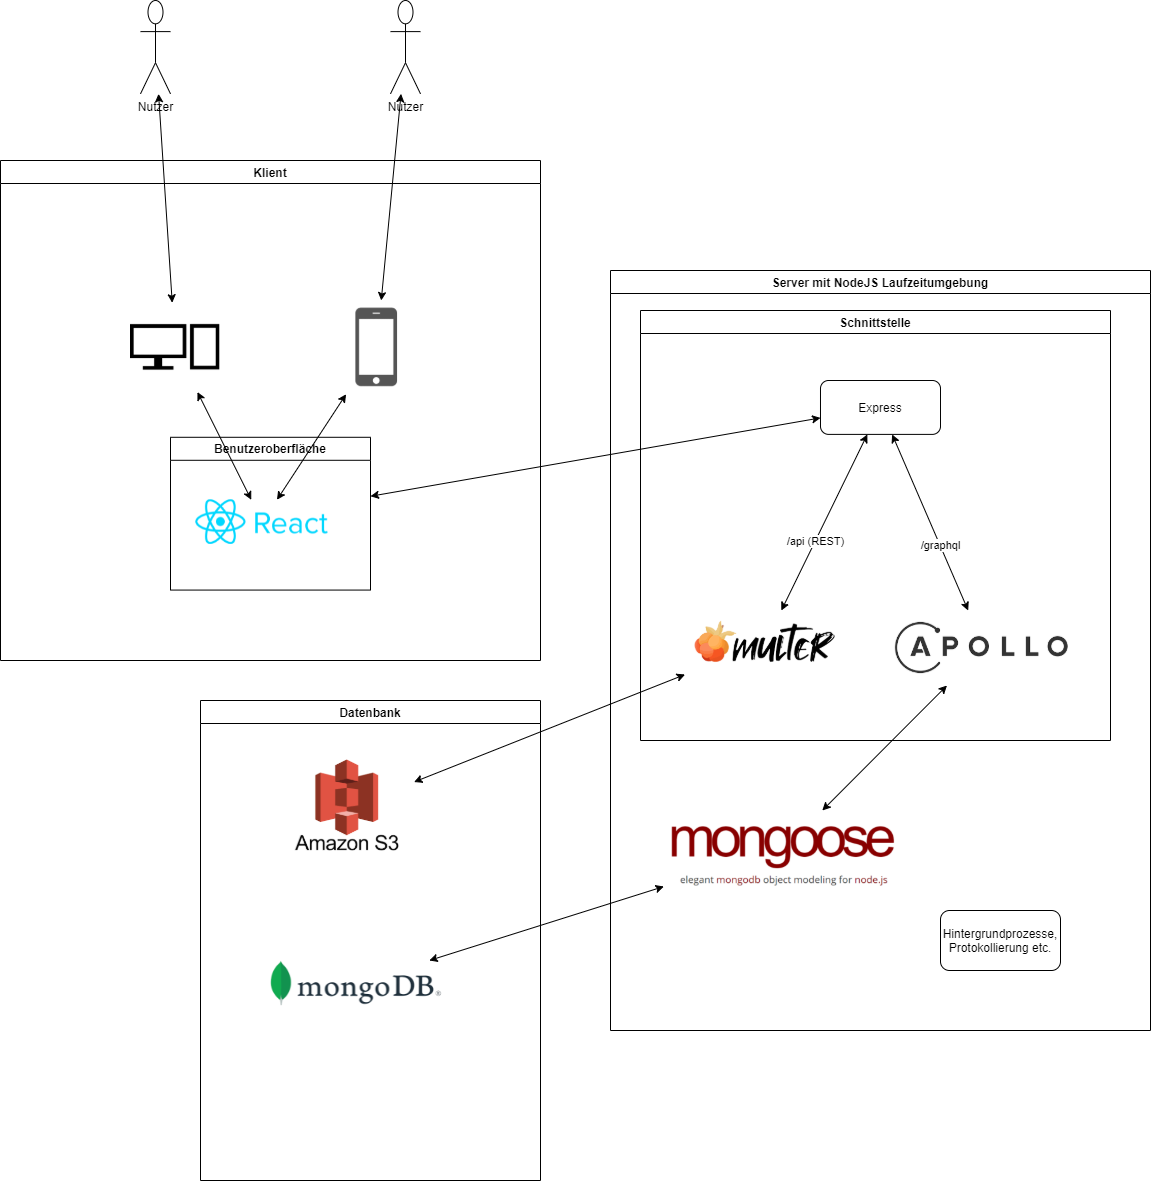
\includegraphics[width=\textwidth]{sources/MERN-Stack_Schaubild.drawio}
\begin{figure}[ht]
	\centering
	\caption{Die Interaktion der verwendeten Technologien als Schaubild}
	\label{figMERN1}
\end{figure}

\paragraph{}
Der Nutzer interagiert mit dessem Endgerät mit der durch React generierten Benutzeroberfläche.
Für dynamische Inhalte werden dazu Anfragen an das NodeJS-Backend gesendet.
Dieses verwaltet mithilfe von Express verschiedene Routen.
Bilder werden als Dateien über die Route \textit{/api} mit Multer auf AWS S3 gespeichert.
Sollten Daten der Datenbank benötigt werden, wird die Route \textit{/graphql} verwendet, bei denen über Apollo und Mongoose die entsprechende Abfrage an die MongoDB-Datenbank geschickt wird. 
Die Technologien sowie dessen Alternativen und die Gründe zur Entscheidung werden in den folgenden Kapiteln erläutert.
